% LTeX: language=de-CH

\section{Methodisches Vorgehen} \label{sec:methodik}

Die vorliegende Arbeit verfolgt ein methodenentwickelndes Ziel: Im Zentrum steht die Konzeption, Umsetzung und Evaluation eines digitalen Erhebungsinstruments zur Analyse des affektiv situativen Wohlbefindens. Dafür wurde eine eigene Smartphone-App (\textit{InterMind}) entwickelt, welche wiederholte, kontextsensitive Befragungen des momentanen Wohlbefindens im Alltag ermöglicht. Methodologisch basiert der Ansatz auf dem Prinzip der \acrfull{esm} sowie deren räumlicher Erweiterung als \acrfull{gema}.

Die entwickelten Instrumente (App und Fragebogen) dienen der Erfassung affektiver Zustände im situativen Kontext, insbesondere mit Blick auf räumliche Umweltfaktoren und soziale Positionierungen. Die so erhobenen Daten werden anschliessend mit Hilfe von \acrfull{maihda} ausgewertet, um intersektionale Effekte auf das subjektive Wohlbefinden modellieren zu können.

Das folgende Kapitel beschreibt zunächst den methodischen Gesamtansatz und begründet die Entscheidung für \acrshort{esm}/\acrshort{gema}. Anschliessend wird die Entwicklung der App dokumentiert, die Durchführung der Datenerhebung beschrieben und die Operationalisierung des Fragebogens erläutert. Abschliessend werden Limitationen des Studiendesigns kritisch reflektiert.


\subsection{Wiederholte Befragung mit \acrshort{esm}, \acrshort{ema} und \acrshort{gema}}

Die systematische Erhebung von momentanen Wohlbefindenszuständen erfordert Methoden, die subjektive Erfahrungen möglichst unmittelbar und kontextspezifisch erfassen. Retrospektive Selbstauskünfte sind hierfür nur begrenzt geeignet, da sie Verzerrungen durch selektive Erinnerung oder nachträgliche Neubewertung unterliegen (\textit{Recall Bias}) \parencite{kahnemanDevelopmentsMeasurementSubjective2006}. Um solche Verzerrungen zu vermeiden, wurde bereits in den 1980er-Jahren die \acrfull{esm} entwickelt. Dieses Verfahren basiert auf der mehrfach wiederholten Erhebung subjektiver Zustände im Alltag – etwa durch zufällig verteilte Signale, die Teilnehmende dazu auffordern, ihre momentane Stimmung, Tätigkeit oder Umgebung zu protokollieren \parencite{csikszentmihalyiValidityReliabilityExperienceSampling1987}. Ziel ist es, das Erleben möglichst nah am Zeitpunkt der Erfahrung und im natürlichen Kontext zu erfassen.

Während \acrshort{esm} ursprünglich als psychologisches Messinstrument konzipiert war, wurde der Ansatz in den 1990er-Jahren durch das Konzept der \acrfull{ema} methodologisch erweitert. \acrshort{ema} bezeichnet nicht nur die unmittelbare Erhebung subjektiven Erlebens, sondern schliesst auch physiologische, verhaltensbezogene oder kontextuelle Daten mit ein – etwa über mobile Geräte, Sensorik oder Tagebuchsysteme \parencite{shiffmanEcologicalMomentaryAssessment2008}. Der Begriff „ökologisch“ verweist hierbei nicht auf natürliche Umwelt, sondern auf den Anspruch, Erleben und Verhalten im realweltlichen Lebenskontext zu erfassen – also dort, wo es tatsächlich stattfindet.

Mit der zunehmenden Verbreitung von GPS-fähigen Endgeräten wurde \acrshort{ema} in den 2010er-Jahren durch das Konzept der \acrfull{gema} ergänzt. \acrshort{gema} kombiniert die subjektive Momentaufnahme mit objektiven, räumlich verortbaren Kontextinformationen wie Standort, Wetter, Lärm oder Bebauungsstruktur \parencite{kirchnerSpatiotemporalDeterminantsMental2016}. Im Unterschied zu \acrshort{ema} liegt der Fokus hier auf der systematischen räumlichen Verknüpfung: Subjektive Erfahrungen werden nicht nur als situativ, sondern explizit als räumlich situiert begriffen. Entscheidend ist dabei nicht die Art der Umgebung – also ob es sich etwa um Grünflächen, urbane Plätze oder Transiträume handelt –, sondern die Möglichkeit, affektives Erleben in seiner Beziehung zum jeweils spezifischen räumlich-materiellen Kontext zu analysieren.

Die vorliegende Arbeit folgt diesem methodischen Paradigma. Ziel ist es, situativ affektive Zustände im Raum nicht nur als individuelle, sondern als kontextuell-räumlich bedingte Erfahrungen zu erfassen. Zu diesem Zweck wurde eine eigene Smartphone-Applikation (\textit{InterMind}) entwickelt, die Teilnehmende mehrmals täglich dazu auffordert, eine kurze Selbsteinschätzung ihres momentanen Wohlbefindens und ihrer Umgebungvorzunehmen. Gleichzeitig werden automatisiert Geodaten gespeichert, sodass jede Beobachtung in ihrer konkreten räumlichen Verortung analysiert werden kann. Im Unterschied zu vielen bestehenden GEMA-Studien liegt der Fokus dabei nicht auf spezifischen Umweltmerkmalen wie Vegetationsanteil oder Luftqualität, sondern auf der relationalen Analyse von Raum und subjektivem Erleben.

Die Entscheidung für ein solches Studiendesign bringt gegenüber querschnittbasierten Verfahren mehrere methodische Vorteile mit sich. Erstens reduziert die wiederholte intraindividuelle Erhebung Verzerrungen durch retrospektive Einschätzungen und erlaubt eine präzisere Erfassung situativer Schwankungen. Zweitens ermöglicht sie eine Kontrolle individueller Basisniveaus, was insbesondere für intersektionale Analysen relevant ist, die sowohl zwischen als auch innerhalb von Personen Differenzierungen vornehmen. Drittens erlaubt die Kombination von Echtzeitbefragung und Geodatenanalyse eine kontextsensitive Modellierung der Beziehungen zwischen affektivem Zustand und Umgebung – im Sinne eines relationalen, ökologisch verstandenen Raumbegriffs \parencite{mascherekMeadowsAsphaltRoad2025}.

Für die Erfassung affektiver Zustände wurden numerische Skalen (Slider) eingesetzt als auch Single- und Multiple-Choice-Fragen, die sich in bisherigen Studien als verlässlich und teilnehmendenfreundlich erwiesen haben \parencite{cookeMeasuringWellBeingReview2016}. Die räumliche Verortung erfolgte einerseits über Single- und Multiple-Choice-Fragen, die sich auf die Umgebung des Teilnehmenden beziehen, und andererseits über die Standortdaten der Smartphone-App, wodurch sich subjektive Einschätzungen und objektive Kontextdaten präzise miteinander verknüpfen lassen. Die methodische Grundlage dieser Studie lässt sich somit als eine kritische Anwendung von \acrshort{gema} verstehen, die affektives Wohlbefinden nicht als isolierte Innenwelt, sondern als kontextgebundenes Erleben in Wechselbeziehung von Raum, Situation und sozialer Positionierung begreift.

\subsection{Methodenentwickelnder Charakter und illustrativer Testdurchlauf} \label{sec:methodenentwickelnd}

Diese Arbeit ist als methodenentwickelnde Studie konzipiert. Im Zentrum steht die Entwicklung eines digitalen Erhebungsinstruments, das die situative Erfassung von affektivem Wohlbefinden mit einer intersektionalen Analyse verknüpft. Ziel ist es, einen vollständigen methodischen Workflow zu entwerfen – bestehend aus einem spezifisch konzipierten Fragebogen, einer Smartphone-Applikation zur standortbezogenen Datenerhebung sowie einer vorbereiteten Analysestruktur für für eine intersektionale Modellierung.

Im Unterschied zu klassischen empirischen Studien liegt der Fokus auf der konzeptionellen und technischen Umsetzbarkeit des Ansatzes. Die wenigen im Rahmen der Pilotstudie erhobenen Daten dienen ausschliesslich der Erprobung und exemplarischen Durchführung des methodischen Prozesses – sie erlauben aufgrund der geringen Stichprobengrösse keine  Aussagen über Zusammenhänge zwischen Umgebung, intersektionaler Positionierung und Wohlbefinden.

Die Durchführung einer \acrshort{maihda}-Analyse erfolgt demnach lediglich zu illustrativen Zwecken. Sie diente dazu, die Struktur des Modells zu testen, die Anforderungen an die Datenqualität und -quantität zu reflektieren und das methodische Zusammenspiel von Erhebungsdesign und Analyseansatz zu überprüfen. Auch andere Auswertungsschritte – etwa deskriptive Statistiken oder Visualisierungen – verfolgen keine analytische Zielsetzung im engeren Sinn, sondern dienen der Überprüfung der Funktionsfähigkeit des entwickelten Instruments.

Die methodische Reflexion dieser exemplarischen Anwendung bildet einen zentralen Teil der Arbeit. Sie erlaubt erste Einschätzungen dazu, welche praktischen, technischen oder konzeptionellen Herausforderungen bei der Umsetzung auftreten und wo Anpassungen für künftige Studien notwendig wären. Der wissenschaftliche Mehrwert der Arbeit liegt entsprechend nicht in empirischen Erkenntnissen, sondern in der Bereitstellung und kritischen Diskussion eines erprobten methodischen Zugangs, der für zukünftige Forschungsvorhaben adaptiert und weiterentwickelt werden kann.


\subsection{Vergleich mit bestehenden Erhebungsinstrumenten}

Die im Rahmen dieser Arbeit entwickelte App bewegt sich im Spannungsfeld zweier methodischer Herangehensweisen: der Echtzeiterhebung räumlich kontextualisierter affektiver Zustände (wie bei \textit{Urban Mind}) und der explizit intersektionalen Analyse subjektiver Raumwahrnehmungen (wie bei \textit{Relief Maps+}). Beide bestehenden Instrumente bilden wichtige Referenzpunkte, da sie jeweils zentrale Teilaspekte des hier verfolgten Ansatzes adressieren, jedoch keine vollständige Integration beider Perspektiven vornehmen. Der folgende Vergleich dient dazu, methodische Gemeinsamkeiten und Unterschiede herauszuarbeiten.

\subsubsection{Urban Mind: \acrshort{gema} ohne intersektionale Perspektive}

Das \textit{\gls{urbanmind}}-Projekt\footnote{Siehe \href{https://www.urbanmind.info/}{urbanmind.info}} stellt ein beispielhaftes Werkzeug dar, um subjektives momentanes Wohlbefinden in städtischen Kontexten mittels Echtzeiterhebungen systematisch zu erfassen und zu analysieren \parencite{bakolisUrbanMindUsing2018}. Es basiert auf einer mobilen Smartphone-App, die mithilfe von \acrshort{gema} detaillierte Einblicke in den Zusammenhang zwischen unmittelbaren Umweltfaktoren und psychischer Gesundheit ermöglicht.

Zentrales Anliegen des \textit{Urban Mind}-Tools ist es, die Effekte spezifischer natürlicherElemente der Umgebung, wie beispielsweise Bäume, Himmel, Wasser oder Vogelgesang, auf die psychische Gesundheit in Echtzeit zu untersuchen. Hierfür werden Proband\genderstern innen mehrmals täglich über einen Zeitraum von zwei Wochen aufgefordert, kurze standardisierte Fragen zu ihrer aktuellen Umgebung und ihrem momentanen Wohlbefinden zu beantworten \parencite{bakolisUrbanMindUsing2018}. Die Datenerhebung erfolgt sowohl mittels Selbsteinschätzungen der räumlichen und sozialen Umgebung als auch über Geodaten, welche automatisiert die exakte räumliche Verortung der Teilnehmer\genderstern innen ermöglichen.

\begin{figure}[h]
    \centering
    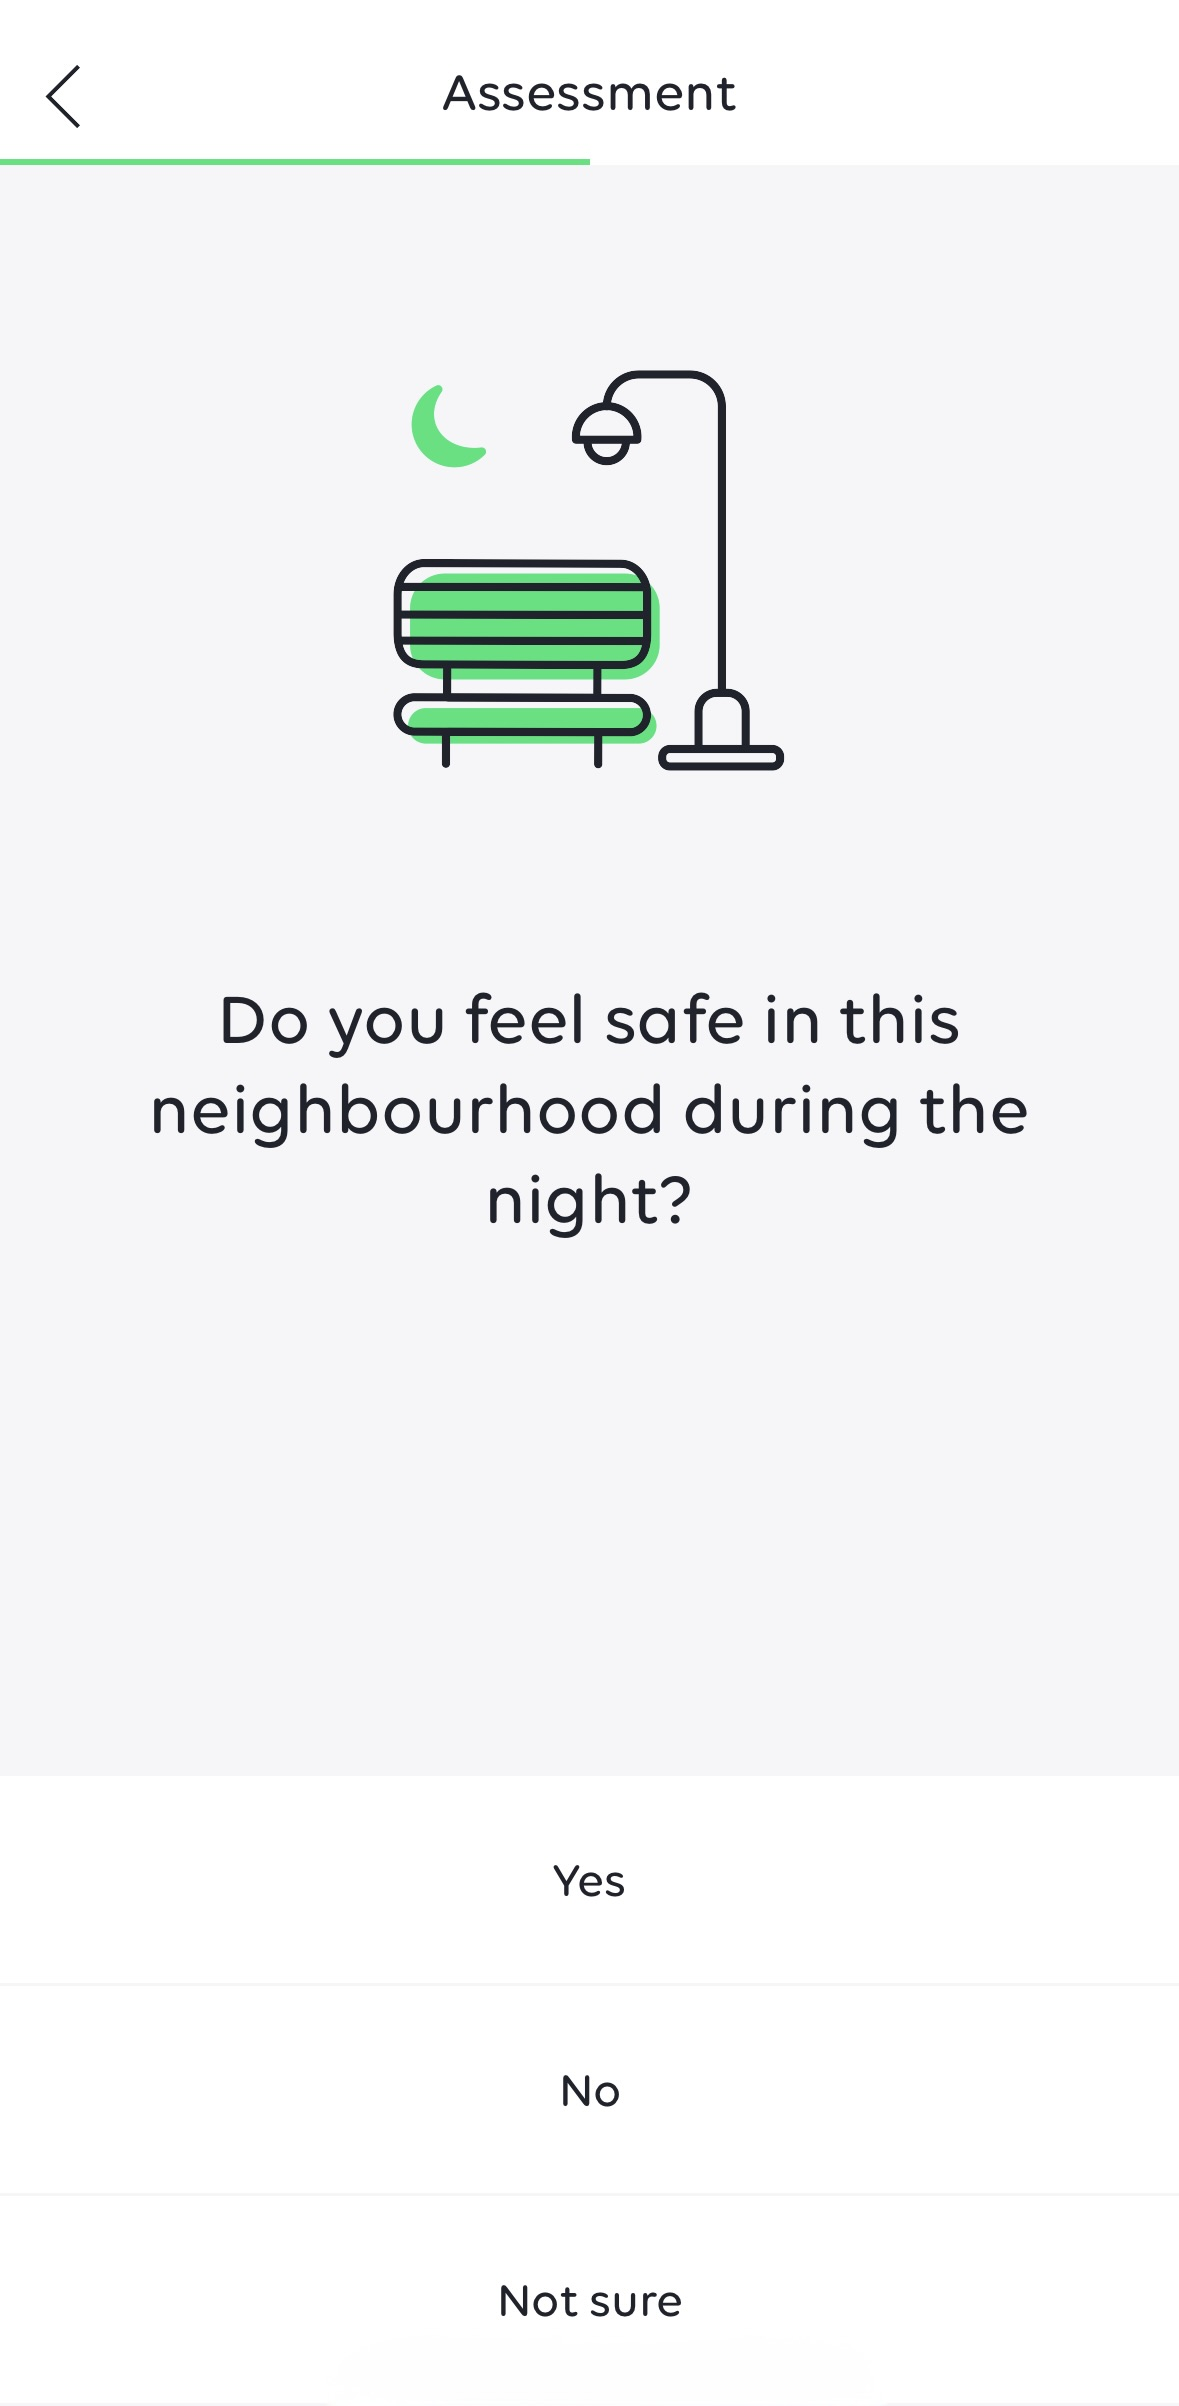
\includegraphics[width=0.3\textwidth]{Arbeit/images/urban_mind01.jpeg}
    \caption{Screenshot einer typischen Frageseite aus der Urban Mind-App}
    \label{fig:urban_mind_screenshot_1}
\end{figure}

Im Gegensatz zu traditionellen querschnittlichen Designs erlaubt das Urban Mind-Tool explizit die Analyse unmittelbarer und zeitverzögerter Effekte (Lag-Effekte). So konnten beispielsweise signifikant positive Effekte von natürlichen Elementen wie Vogelgesang oder dem Vorhandensein von Bäumen auf das momentane Wohlbefinden nachgewiesen werden, welche auch mehrere Stunden nach dem eigentlichen Kontakt noch messbar waren \parencite{bakolisUrbanMindUsing2018}. Darüber hinaus betont das Tool die Bedeutung individueller Differenzen und psychologischer Charakteristika, wie beispielsweise Impulsivität, die sich als moderierende Variable herausstellte: Personen mit höherer Impulsivität, welche typischerweise ein erhöhtes Risiko für psychische Erkrankungen aufweisen, profitieren stärker von unmittelbaren Naturerfahrungen.

Hinsichtlich des Designs und der Bedienbarkeit überzeugt die Urban Mind-App durch eine intuitive grafische Gestaltung (siehe \Cref{fig:urban_mind_screenshot_1}) sowie durch motivierende Elemente wie eine visuelle Übersicht über ausgefüllte und verpasste Fragebögen. Zudem ermöglicht sie Nutzer\genderstern innen, ihre eigenen Daten retrospektiv aufzubereiten, was zu einer angeleiteten Reflexion des eigenen Wohlbefindens beiträgt. Dieses Feature unterstützt insbesondere eine nachhaltige und motivierte Teilnahme über den gesamten Erhebungszeitraum hinweg.

Obwohl Urban Mind zahlreiche methodische und technische Stärken aufweist, berücksichtigt es intersektionale Perspektiven bisher nicht explizit. So sind beispielsweise soziale Kategorien wie Geschlecht, Ethnizität oder sozioökonomischer Status zwar als demografische Variablen erfasst, werden jedoch nicht systematisch in einer intersektionalen Analyse miteinander in Beziehung gesetzt. Theoretisch wäre es möglich, intersektionale Analysen retrospektiv auf Grundlage der erhobenen Daten durchzuführen, eine solche methodische Perspektive wurde jedoch bislang nicht verfolgt.

\subsubsection{Relief Maps+: Reflexive und intersektionale Kartierung retrospektiver Erfahrungen}

Im Unterschied zu Echtzeit-Tools wie „Urban Mind“, die affektives Wohlbefinden situativ-erlebensnah quantifizieren, verfolgt \textit{\gls{reliefmaps}}\footnote{Siehe \href{https://reliefmaps.upf.edu/}{reliefmaps.upf.edu}} einen qualitativ-reflexiven Ansatz, der retrospektiv subjektive Erfahrungen intersektional positioniert sichtbar macht \parencite{rodo-de-zarateDevelopingGeographiesIntersectionality2014}. Aufbauend auf der ursprünglichen Version der „Relief Maps“ integriert die digitale Anwendung drei miteinander verschränkte Dimensionen – geografische Orte, soziale Identitäten und emotionale Bewertungen – und legt dabei besonderen Wert auf die Förderung individueller Selbstreflexion und kollektiver Sichtbarmachung diskriminierender Raumstrukturen.

Zu Beginn des Erhebungsprozesses erstellen Nutzer\genderstern innen einen Avatar auf Basis intersektional relevanter Merkmale wie Geschlecht, Sexualität, Klasse, Herkunft, Körperbild oder (Dis-)Ability. Darauf aufbauend reflektieren sie in mehreren Schritten über emotionale Erfahrungen in verschiedenen Raumkategorien wie „öffentliche Räume“, „Gesundheitseinrichtungen“ oder „virtuelle Räume“ (siehe \cref{fig:relief_maps_plus_screenshot_1}). Für jede Achse sozialer Positionierung können in einem nächsten Schritt Orte je nach erfahrenem (Un-)Wohlsein als unterdrückend, kontrovers, neutral oder entlastend klassifiziert werden. Ergänzend können Orte direkt auf einer Karte verortet und mit freien Kommentaren sowie Emotionslabels wie „Angst“, „Sicherheit“ oder „Empowerment“ versehen werden. Diese Funktion fördert eine dichte, kontextualisierte Beschreibung subjektiver Erlebnisse, die sich nicht auf standardisierte Itemskalen reduzieren lässt.

\begin{figure}[htbp]
    \centering
    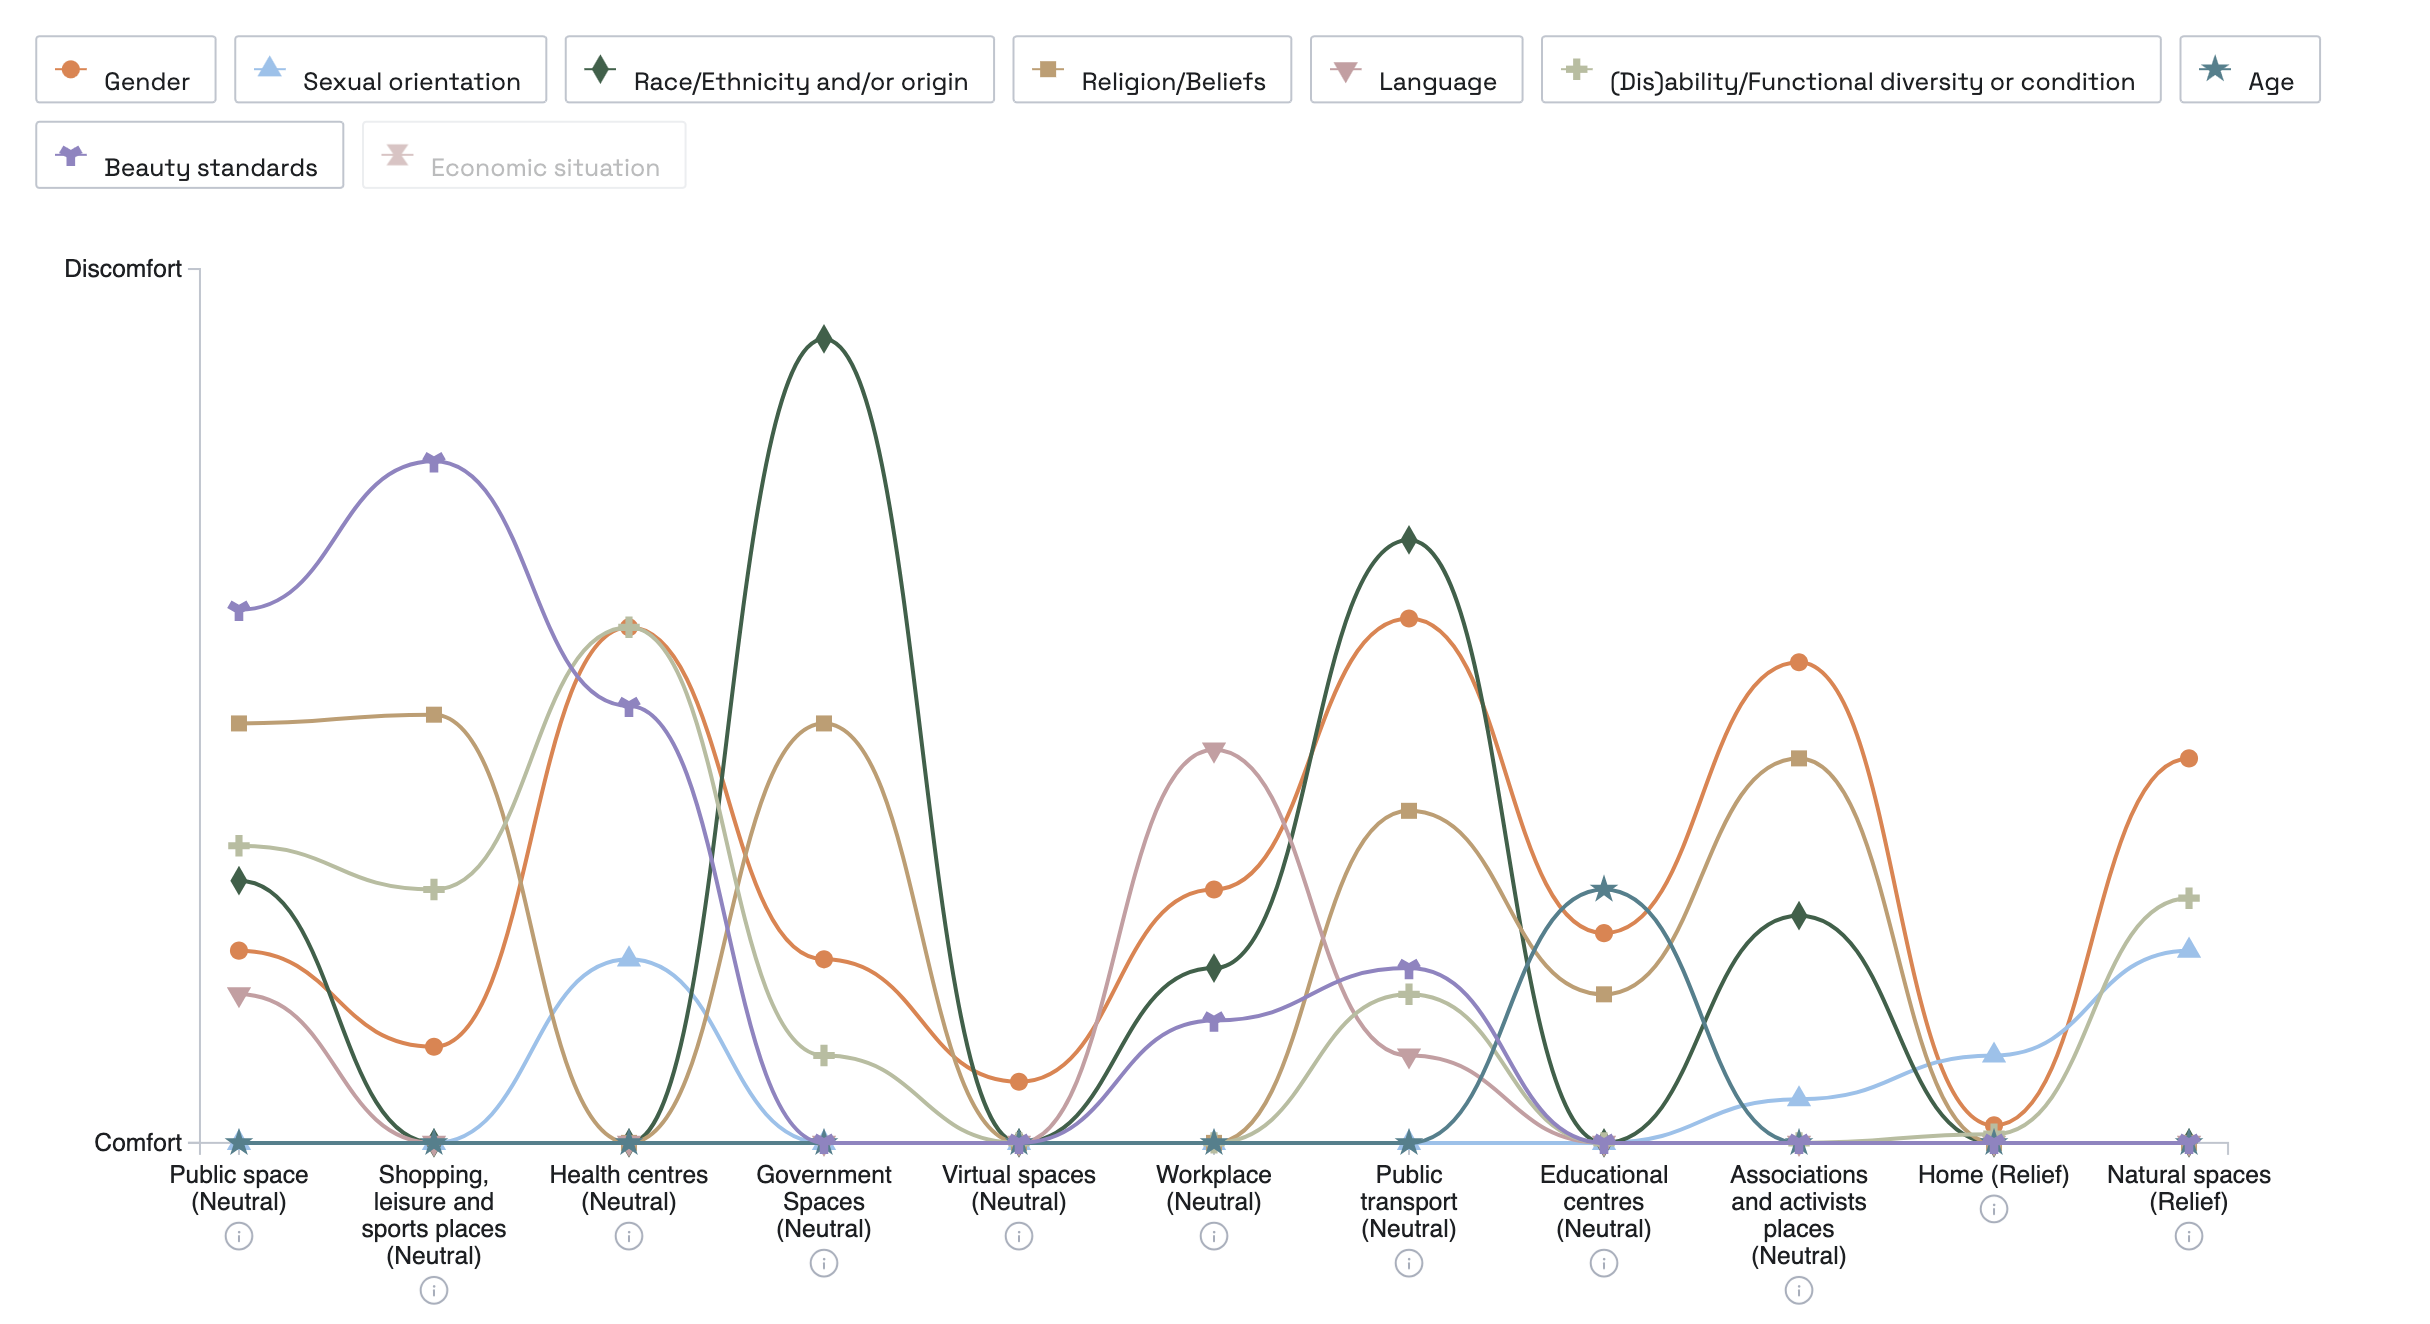
\includegraphics[width=\textwidth]{Arbeit/images/reliefmap.png}
    \caption{Beispielhafte Ausgabe aus dem Relief Maps+ Tool}
    \label{fig:relief_maps_plus_screenshot_1}
\end{figure}

Ein zentrales methodisches Merkmal von Relief Maps+ ist der Versuch, die emotionale Wirkung sozialer Machtverhältnisse räumlich darstellbar zu machen – ohne diese in eindimensionale Kausalbeziehungen zu überführen. Die Nutzer\genderstern innen bewerten ihre Erfahrungen explizit entlang einzelner \glspl{identitaetsachse}. Gleichzeitig zeigt sich hier eine zentrale methodologische Spannung: Die isolierte Betrachtung einzelner Diskriminierungsachsen widerspricht dem Grundgedanken intersektionaler Analyse, der gerade auf die Verwobenheit und Gleichzeitigkeit verschiedener Machtverhältnisse verweist. Eine konsequente intersektionale Operationalisierung bleibt damit methodisch herausfordernd.

Einige technische Merkmale von Relief Maps+ sind auch im Hinblick auf die Entwicklung eigener Tools relevant. Die browserbasierte Anwendung erlaubt es Forschenden, eigenständig Projekte zu erstellen und auszuwerten. Allerdings ist der Zugang derzeit stark auf den katalanischen Kontext zugeschnitten: Verfügbare Sprachen sind Katalanisch, Spanisch und Englisch; Optionen zur Erweiterung oder Lokalisierung sind nicht dokumentiert. Da der Quellcode nicht öffentlich zugänglich ist, bleiben Fragen zur Anpassbarkeit, Wiederverwendbarkeit und langfristigen Wartbarkeit offen. Aus methodischer Sicht stellt sich somit die Frage, inwiefern die Software übertragbar ist auf andere sprachliche, kulturelle und geografische Kontexte.

Trotz dieser Einschränkung eröffnet Relief Maps+ wichtige Potenziale: Die bewusste Integration von Reflexivität, die aktive Beteiligung der Nutzer\genderstern innen an der Interpretation ihrer eigenen Erfahrungen sowie die Sichtbarmachung räumlich kontextualisierter Ungleichheiten markieren einen innovativen Zugang für intersektionale, subjektzentrierte Geographien. Die methodische Fundierung des Tools beruht auf einem iterativen Validierungsprozess unter Einbezug feministischer, queerer und dekolonialer Perspektiven \parencite{luizdesouzaSpiralValidationProcess2025}.



\subsubsection{Einordnung des eigenen Ansatzes}

Die im Rahmen dieser Arbeit entwickelte App \textit{InterMind} versteht sich als offen zugängliches und flexibel einsetzbares Werkzeug für Studien im Rahmen der \acrshort{gema}. Ziel war es, eine technisch eigenständige, quelloffene Infrastruktur bereitzustellen, die eine situative, geolokalisierte Erhebung affektiven Wohlbefindens ermöglicht – ein Instrument, das in dieser Form bislang nicht allgemein verfügbar war. Die Entwicklung orientierte sich in Teilen an bestehenden Tools wie \textit{Urban Mind}, insbesondere was das Interface-Design und die Nutzerführung betrifft, basiert jedoch auf einer unabhängig konzipierten Codebasis und wurde vollständig neu implementiert.

Die App selbst ist methodisch nicht innovativ im engeren Sinne, sondern stellt eine robuste, anpassbare Plattform dar, die für verschiedenste \acrshort{gema}-Studien konfiguriert werden kann. Ihr modularer Aufbau erlaubt die Integration beliebiger Fragebögen und Fragetypen – einschliesslich Freitextfeldern, Schiebereglern oder Mehrfachantworten. Damit kann das System flexibel an unterschiedliche Forschungskontexte angepasst und in zukünftigen Studien weiterverwendet werden.

Im Zentrum der vorliegenden Arbeit steht ein spezifisch entwickelter Fragebogen, der auf der App zum Einsatz kommt. Dieser kombiniert klassische \gls{ema}-Items zur situativen Erfassung von Kontext und Wohlbefinden mit explizit intersektional angelegten Fragen. Dabei werden Dimensionen wie Geschlecht, Herkunft oder sozioökonomischer Status getrennt erfasst – ein Ansatz, der zwar theoretisch nicht vollständig der Idee intersektionaler Verwobenheit entspricht, aber eine quantitative Auswertbarkeit ermöglicht. Gleichzeitig bleibt durch offene Antwortformate Raum für reflexive Auseinandersetzung mit der eigenen Erfahrung in konkreten räumlichen Situationen.

\subsection{Entwicklung der App \textit{InterMind}}

Im Zuge dieser Arbeit wurde die App \textit{InterMind} entwickelt, die als technische Grundlage für wiederholte, geolokalisierte und pseudonymisierte Befragungen dient. Sie bildet die Infrastruktur für anschliessend durchgeführte Pilot-Studie. Die App und der in dieser Arbeit eingesetzte Fragenkatalog wurden parallel und iterativ konzipiert. Während dieser Abschnitt die technische Entwicklung der App dokumentiert, wird die inhaltliche Gestaltung des Fragebogens im \cref{sec:fragebogen} erläutert. Der vollständige Quellcode der App ist auf \gls{github}\footnote{\href{https://github.com/lbatschelet/intermind}{https://github.com/lbatschelet/intermind}} veröffentlicht.


\subsubsection{Ziele und Rahmenbedingungen}

Klar machen wieso eine App entwickelt wurde
Klarmachen dass App und Fragebogen nicht dasselbe sind
Weniger labern, weniger wiederholen

sozusagen argumentativ dahin kommen wieso es die app braucht, kann man das analog erheben? nein, kann man das mit vorhandenen tools machen? ja, aber nicht so flexibel wie gewünscht.

stringender formulieren, einleitungstext üb erhaupt zur app entwicklung, dann erst der ganze rest

Die zentrale Erhebungslogik der vorliegenden Arbeit basiert auf wiederholten, geolokalisierten Erhebungen zum situativ-affektiven Wohlbefinden der Teilnehmenden. Daraus resultieren spezifische Anforderungen an das Instrument, mit dem diese Daten erfasst werden sollen. Ein geeignetes Erhebungstool muss insbesondere folgende Kriterien erfüllen: Es soll mobil und einfach nutzbar sein, situative Antworten unmittelbar im Alltag der Teilnehmenden ermöglichen, dabei Standortdaten automatisch erfassen und gleichzeitig datenschutzrechtliche sowie technische Hürden für die Nutzer\genderstern innen minimieren. Darüber hinaus war es von Beginn an wichtig, dass das System flexibel und nachhaltig konzipiert ist, um auch für zukünftige Arbeiten eingesetzt werden zu können. Konkret bedeutet dies, dass die Fragenkataloge sowie die Inhalte der App einfach austauschbar und an neue Forschungsfragen oder Zielgruppen anpassbar sein sollten.

Bereits verfügbare Lösungen erfüllten diese Anforderungen nur teilweise oder gar nicht. Kommerzielle Angebote, wie beispielsweise die Marktforschungsplattform Avicenna\footnote{\href{https://avicennaresearch.com/}{https://avicennaresearch.com/}}, sind aufgrund hoher Lizenzkosten für eine studentische Abschlussarbeit nicht praktikabel. Zudem erlauben viele solcher Dienste in keine vollständige Kontrolle über die verarbeiteten Daten und bieten nur begrenzte Anpassungsmöglichkeiten hinsichtlich Fragenstruktur und Datenerfassung. Auf der anderen Seite stehen Apps wie Urban Mind\footnote{\href{https://urbanmind.info/}{https://urbanmind.info/}}, die zwar grundsätzlich für \gls{gema}-Erhebungen im Forschungskontext entwickelt wurden, jedoch nicht quelloffen und entsprechend auch nicht eigenständig erweiterbar sind. Zudem ist mir persönlich in dieser Arbeit bei der sensible Daten zu Wohlbefinden und sozialen Zugehörigkeiten erhoben werden, eine transparente und sichere Datenverarbeitung von besonderer Bedeutung.

Vor diesem Hintergrund wurde das Ziel formuliert, eine eigene digitale Anwendung zu entwickeln, die bewusst quelloffen und modular gestaltet ist. Diese \gls{opensource}-Architektur sollte es ermöglichen, die gesamte Datenverarbeitung transparent und nachvollziehbar zu gestalten sowie künftige Anpassungen unkompliziert vorzunehmen. Aufgrund der limitierten zeitlichen Ressourcen innerhalb der Bachelorarbeit wurde darüber hinaus darauf geachtet, weit verbreitete Technologien und Frameworks zu wählen, um die Entwicklung möglichst effizient, wartungsarm und für Dritte nachvollziehbar zu halten.

\subsubsection{Konzeptionsphase}
Auf Basis der beschriebenen Anforderungen wurde zunächst ein detaillierter Anforderungskatalog entwickelt, der als zentraler Leitfaden für die weiteren Schritte der Entwicklung diente. Dieser Katalog wurde iterativ ergänzt, konkretisiert und während des gesamten Entwicklungsprozesses kontinuierlich an methodische und technische Erkenntnisse angepasst. In Anlehnung an etablierte Konzepte aus der Softwareentwicklung wurde dabei zwischen funktionalen und nicht-funktionalen Anforderungen unterschieden.

Funktionale Anforderungen definieren dabei konkret, \textit{was} die App im praktischen Einsatz leisten muss, und legen somit die notwendigen Funktionen und Abläufe der Anwendung fest. Für diese Studie bedeutete dies insbesondere, dass die App den Teilnehmenden täglich drei zufällig über den Tag verteilte Beantwortungszeiträume von einer Stunde ermittelt und jeweils zum Start dieser Zeiträume \glspl{pushnotification} sendet. Diese Anforderung schloss bereits früh eine Browser-basierte Erhebung aus, und führte zum Entscheid eine App-basierte Erhebung zu wählen. Weiter wurde festgelegt, dass bei jeder erfolgten Befragung der aktuelle Standort automatisiert mit erfasst werden soll, sofern die Teilnehmenden dies technisch erlauben. Um die Erhebung flexibel und bedarfsgerecht zu gestalten, wurden zudem verschiedene Fragetypen vorgesehen, darunter Single-Choice, Multiple-Choice, Skalen-basierte Fragen (Slider) sowie Freitextfelder. Schliesslich wurde es als zwingende funktionale Anforderung definiert, dass Teilnehmende jederzeit eigenständig sämtliche gespeicherten Daten löschen können. Die Teilnahme erfolgt dabei vollständig anonym, über eine gerätegebundene, automatisch generierte pseudonyme \gls{uuid}, ohne jegliche Form der Registrierung oder der Eingabe personenbezogener Daten.
 
Nicht-funktionale Anforderungen legen hingegen fest, \textit{wie} diese Funktionen umgesetzt werden sollen, und beschreiben qualitative Merkmale wie Sicherheit, Benutzerfreundlichkeit oder technische Kompatibilität. In diesem Projekt wurden insbesondere Datenschutz und Datensicherheit als zentrale nicht-funktionale Anforderungen definiert. Sämtliche Datenverarbeitungsprozesse müssen entsprechend den Vorgaben des \acrfull{dsg} und der Europäischen Datenschutzgrundverordnung \acrshort{dsgvo} erfolgen. Weiterhin wurde Mehrsprachigkeit (Deutsch, Englisch und Französisch) als Voraussetzung formuliert, ebenso wie die Möglichkeit einer späteren Erweiterung auf weitere Sprachen. Darüber hinaus sollte die Anwendung ursprünglich grundsätzlich offlinefähig sein. Im laufe der Entwicklung wurde diese Anforderung jedoch aufgegeben, da das dazu geführt hätte, dass jede Änderung im Fragenkatalog ein Update der App und anschliessend je nachdem nicht kompatible Versionen der App entstünden. Um Teilnehmenden mit unterschiedlichen Mobilgeräten die Teilnahme möglichst einfach zu machen, war zudem eine plattformübergreifende Kompatibilität für  und Android erforderlich. Schliesslich war eine offene, modulare und nachvollziehbare Codebasis wichtig, sodass Anpassungen und Erweiterungen des Systems durch andere Forschende mit minimalem Aufwand möglich bleiben. Dies wurde dadurch erreicht, dass die App als \gls{opensource}-Projekt auf \gls{github}\footnote{\href{https://github.com/lbatschelet/intermind}{https://github.com/lbatschelet/intermind}} veröffentlicht wurde.

Die Priorisierung und Auswahl dieser Anforderungen erfolgte unter Berücksichtigung der konkreten Forschungsziele, der vorhandenen Literatur zu mobilen Anwendungen im Bereich \gls{esm}/\gls{gema} \parencite[u.a.][]{chenPerceivedUrbanEnvironment2025, bakolisUrbanMindUsing2018, randallDevelopmentTrialMobile2013}, datenschutzrechtlicher Vorgaben sowie praktischer Erfahrungen aus dem eigenen Studium. Aufgrund des iterativen Vorgehens während der Entwicklung kam es dabei auch später immer wieder zu Anpassungen und Nachjustierungen einzelner Anforderungen.

\subsubsection{Datenschutz als Gestaltungsprinzip}

Datenschutz spielte von Beginn an eine zentrale Rolle im Entwicklungsprozess und beeinflusste sowohl die technische Architektur als auch methodische Entscheidungen. Es wird konsequent dem Prinzip \textit{Privacy by Design} gefolgt, das vorsieht, Datenschutzanforderungen bereits bei der Konzeption einer Anwendung mitzudenken und nicht nachträglich zu ergänzen \parencite{cavoukianPrivacyDesign72009}. Ziel ist es, ein hohes Mass an Privatsphäre zu gewährleisten und gleichzeitig volle Transparenz über die Erhebung und Verarbeitung der Daten sicherzustellen.

In der Umsetzung wurde das Prinzip \textit{Privacy by Design} konkret durch technische Massnahmen wie \textit{privacy by architecture} realisiert \parencite{spiekermannEngineeringPrivacy2009}. Die App erfasst keine personenbezogenen Angaben wie Namen, Telefonnummern oder E-Mail-Adressen. Stattdessen wird beim ersten Start automatisch eine gerätegebundene \glsfirst{uuid} generiert, über die alle Daten pseudonymisiert zugeordnet werden. Eine kontinuierliche Ortung findet nicht statt; Standortdaten werden ausschliesslich zum Zeitpunkt einer beantworteten Befragung erhoben.


Die Speicherung der Daten erfolgt auf einem Server in der Schweiz unter Verwendung der Plattform \gls{supabase} und einer \gls{postgresql}-\gls{datenbank}. Eine Zugriffskontrolle auf Zeilenebene (\gls{rls}) stellt sicher, dass jedes Endgerät nur auf die eigenen Daten zugreifen kann. Alle Datenübertragungen zwischen App und Server sind verschlüsselt und erfolgen über authentifizierte Schnittstellen.

Teilnehmende können ihre Datensätze jederzeit direkt über die App löschen. Damit werden sämtliche Einträge, die mit ihrer \gls{uuid} verknüpft sind, dauerhaft entfernt. Die Kontrolle über die eigenen Daten bleibt somit vollständig bei den Nutzer\genderstern innen.

Alle datenschutzrelevanten Aspekte sind in einer eigenen Datenschutzrichtlinie dokumentiert, die über die App sowie auf der Projektwebseite\footnote{\href{https://intermind.ch/privacy-policy.html}{https://intermind.ch/privacy-policy.html}} öffentlich zugänglich ist. Die Richtlinie erläutert zudem die Rechte der Teilnehmenden nach Schweizer Datenschutzgesetz (\gls{dsg}) und der Europäischen Datenschutzgrundverordnung (\gls{dsgvo}).


\subsubsection{Implementierung}

Die technische Umsetzung orientierte sich an etablierten Prinzipien des Software Engineerings \parencite{sommervilleSoftwareEngineering2016} sowie an den zentralen Gestaltungsprinzipien von \gls{solid} \parencite{martinAgileSoftwareDevelopment2002}. Im Zentrum standen dabei eine saubere Trennung zwischen Anwendungslogik, Datenhaltung und Benutzeroberfläche, eine modulare Struktur der Komponenten sowie eine klare Zuordnung von Verantwortlichkeiten.

Für die Umsetzung wurde das \gls{framework} \gls{reactnative} in Kombination mit der Entwicklungsplattform \gls{expo} gewählt. Diese Entscheidung ermöglichte es, mit einer einheitlichen Codebasis sowohl \gls{ios}- als auch \gls{android}-Geräte zu unterstützen. Dadurch reduzierte sich der Entwicklungsaufwand, während gleichzeitig eine konsistente Benutzererfahrung auf beiden Plattformen sichergestellt werden konnte. Als serverseitige Infrastruktur kam \gls{supabase} zum Einsatz – ein \gls{opensource} \gls{backend}-as-a-Service auf Basis einer relationalen \gls{postgresql}-\gls{datenbank}, das \gls{authentifizierung}, \gls{autorisierung}, Datenspeicherung und sichere Datenübertragung integriert bereitstellt.

Der Fragenkatalog ist nicht im Quellcode verankert, sondern wird dynamisch über eine \gls{json}-Konfigurationsdatei aus der \gls{datenbank} geladen. Dadurch können Inhalte ohne App-Update angepasst werden, was weitestgehend verhindert, dass inkompatible Versionen der App entstehen. Diese Flexibilität erfordert jedoch eine aktive Internetverbindung für das Laden der Befragungsinhalte.

Nach dem erstmaligen Ausfüllen eines Fragebogens berechnet die App automatisch drei individuelle und zufällige Befragungszeitpunkte pro Tag. Diese werden lokal auf dem Gerät gespeichert. Die Zeitpunkte werden täglich zufällig innerhalb von drei Tagesabschnitten (Morgen, Mittag/Nachmittag, Abend) gewählt. Ein Mindestabstand zwischen den einzelnen Befragungen garantiert eine gleichmässige zeitliche Verteilung. Sobald ein Zeitpunkt erreicht ist, erhalten die Teilnehmenden eine Benachrichtigung und haben ab diesem Moment exakt eine Stunde Zeit, um den Fragebogen auszufüllen. Wird der Fragebogen nicht innerhalb dieser Zeitspanne ausgefüllt, verfällt der Slot und die App schickt eine weitere Benachrichtigung beim nächsten geplanten Zeitpunkt.

Das \gls{frontend} wurde minimalistisch und funktional gestaltet, um eine intuitive Nutzung zu ermöglichen und eine möglichst neutrale Darstellung der Fragen sicherzustellen \parencite{rogersInteractionDesignHumancomputer2023}. Die App gliedert sich in drei Hauptbereiche: einen Startbildschirm mit dem nächsten Befragungszeitfenster, den Fragebogenbereich und einen Informations- und Einstellungsbildschirm mit Hinweisen zum Datenschutz. Zur visuellen Unterstützung wurden generische \gls{opensource}-Vektorgrafiken von Katerina Limpitsouni\footnote{\href{https://undraw.co/}{undraw.co/}} verwendet.


\subsubsection{Test und Iteration}
Zur Sicherstellung der technischen Zuverlässigkeit sowie der Gebrauchstauglichkeit der App wurde im Rahmen dieser Arbeit ein zweistufiger Testprozess durchgeführt. Aufgrund der begrenzten Ressourcen und des Projektumfangs kam dabei keine strukturierte automatisierte Testsuite zum Einsatz. Stattdessen wurde ein pragmatischer Ansatz gewählt, bei dem auftretende Probleme laufend manuell identifiziert und unmittelbar behoben wurden. Obwohl diese Vorgehensweise zu einer insgesamt soliden Funktionalität der Anwendung führte, erwies sich die fehlende automatisierte Qualitätssicherung im Entwicklungsprozess wiederholt als Herausforderung und führte zu einem insgesamt höheren zeitlichen Aufwand bei der Fehlersuche.

In einer ersten Phase fanden fortlaufende technische Funktionstests während der Implementierung statt. Im Fokus dieser Tests standen insbesondere die korrekte Verarbeitung des dynamisch geladenen Fragenkatalogs (\gls{json}-Datei), die fehlerfreie Übertragung von Daten an das \gls{supabase}-\gls{backend}, das Verhalten der App bei unterbrochener oder unzuverlässiger Internetverbindung sowie die plattformübergreifende Zuverlässigkeit der lokalen Planung und Ausführung von \glspl{pushnotification}. Da sich iOS und Android in ihrer Handhabung von Hintergrundprozessen, Benachrichtigungssystemen und Berechtigungsanfragen teilweise stark unterscheiden, wurde der Funktionsumfang regelmässig auf verschiedenen Geräten mit unterschiedlichen Betriebssystemversionen manuell geprüft.

In der zweiten Phase wurde ein interner Pretest mit vier Personen durchgeführt, welche die App über einen Zeitraum von zwei Wochen nutzten. Die Teilnehmenden erhielten hierzu über die offiziellen Beta-Testplattformen (TestFlight für iOS und Google Play Console für Android) Zugang zur Anwendung. Dabei wurden gezielte Aufgaben gestellt, um spezifische technische und inhaltliche Aspekte zu überprüfen sowie allgemeines Feedback zur Benutzerfreundlichkeit und Verständlichkeit der Fragen zu sammeln. Die Rückmeldungen der Testpersonen bezogen sich vor allem auf die Klarheit und Lesbarkeit einzelner Fragen und Texte, auf kleinere Probleme bei der erstmaligen Vergabe von App-Berechtigungen (z. B. Standortzugriff), sowie auf Darstellungsprobleme bestimmter \gls{ui}-Elemente auf verschiedenen Geräten.

Die Ergebnisse aus dieser Testphase führten sowohl zu technischen Anpassungen als auch zu inhaltlichen Änderungen im Fragebogen. Mehrere Fragen wurden sprachlich präzisiert oder gekürzt, einzelne Items wurden ganz gestrichen. Weiterhin wurden Anpassungen an der Benutzeroberfläche vorgenommen, beispielsweise bei Abständen und der Platzierung von Slider-Beschriftungen. Aufgrund der fehlenden automatisierten Tests erforderte jede Änderung erneut eine manuelle Überprüfung der gesamten Funktionalität, was insgesamt erheblichen zusätzlichen Aufwand bedeutete.

Insgesamt ermöglichte der iterative Testprozess jedoch, wesentliche Schwachstellen vor dem Beginn der eigentlichen Datenerhebung zu identifizieren und zu beheben. Obwohl auf eine formalisierte Usability-Evaluation verzichtet wurde, konnten durch diese Vorgehensweise zentrale technische sowie benutzerorientierte Probleme effektiv adressiert werden.

\subsubsection{Veröffentlichung und Distribution}

Um die entwickelte App für die eigentliche Datenerhebung nutzen zu können, wurde eine Veröffentlichung über die offiziellen App-Stores von Apple (iOS) und Google (Android) angestrebt. Beide Plattformen stellen dabei unterschiedliche technische, administrative und finanzielle Anforderungen, die den Veröffentlichungsprozess massgeblich beeinflussten.

Die Veröffentlichung im Apple App Store setzte zunächst den Erwerb einer kostenpflichtigen Entwicklerlizenz voraus, für die eine jährliche Gebühr von CHF 100 zu entrichten war. Nach erfolgreicher Einrichtung dieses Entwicklerkontos wurde die App zur Veröffentlichung eingereicht, allerdings von Apple zunächst nicht für eine finale Veröffentlichung im regulären App Store zugelassen. Als Begründung wurde angegeben, die App weise zu wenig inhaltlichen Mehrwert auf – eine Entscheidung, die aus Sicht der Entwicklung nur schwer nachvollziehbar war. Der Prüfprozess bei Apple ist zum Zeitpunkt des Abschlusses dieser Arbeit noch nicht vollständig abgeschlossen. Dennoch konnte die App über Apples eigene Plattform für öffentliche Beta-Tests („TestFlight“) bereitgestellt werden, sodass Teilnehmende der Studie über einen offiziellen TestFlight-Link Zugang zur App erhielten.

Im Gegensatz dazu verlangte Google für eine Veröffentlichung im Android Play Store keine laufenden Lizenzkosten. Allerdings stellte Google die Bedingung, dass vor einer offenen Betaversion zunächst ein geschlossener Test mit mindestens 20 Personen über einen Zeitraum von zwei Wochen durchgeführt werden musste. Da es innerhalb des zeitlichen Rahmens dieser Bachelorarbeit nicht möglich war, eine ausreichende Anzahl Testpersonen mit Android-Geräten zu rekrutieren, wurde hierfür ein externer Dienstleister in Anspruch genommen, welcher diesen erforderlichen Test für eine Gebühr von CHF 30 durchführte. Nach erfolgreichem Abschluss dieses Tests wurde die App im Play Store als offene Beta veröffentlicht und war somit öffentlich verfügbar.

Darüber hinaus verlangten beide Plattformen, dass eine öffentlich zugängliche Datenschutzrichtlinie zur Verfügung steht. Zu diesem Zweck wurde die Website intermind.ch eingerichtet, auf der neben der vollständigen Datenschutzerklärung auch ergänzende Informationen zum Forschungshintergrund abrufbar sind. Die Kosten hierfür beliefen sich auf einmalig CHF 10 für die Domainregistrierung; Hosting-Kosten entstanden keine zusätzlichen, da auf bereits bestehende Infrastruktur zurückgegriffen wurde.

Durch die Veröffentlichung über offizielle App-Plattformen konnten technische Hürden für die Teilnehmenden minimiert und zugleich plattformspezifische Anforderungen (beispielsweise hinsichtlich Datenschutzrichtlinien und Update-Management) zuverlässig erfüllt werden. Trotz vereinzelter Schwierigkeiten im Freigabeprozess ermöglichte dieses Vorgehen letztlich eine unkomplizierte Distribution und Nutzung der Anwendung im Rahmen dieser Arbeit.

\subsection{Fragebogenentwicklung}\label{sec:fragebogen}

Der Fragebogen besteht aus zwei zentralen Elementen:

\paragraph{Baseline-Befragung (einmalig):}
Hier wurden grundlegende demografische Variablen (Alter, Geschlecht, sexuelle Orientierung, Behinderung, sozioökonomischer Hintergrund) erhoben, um soziale Positionierungen für spätere intersektionale Analysen verfügbar zu machen. Fragen wurden bewusst offen oder mit freier Spezifikation gestaltet, um Normativität in den Antwortoptionen zu vermeiden und soziale Positionierungen differenziert erfassen zu können.

\paragraph{Situative Befragung (wiederholt):}
Der wiederholt eingesetzte Fragebogen besteht aus kurzen situativen Erhebungen, die mittels EMA durchgeführt wurden. Teilnehmer:innen wurden regelmässig aufgefordert, Fragen zu ihrem momentanen Wohlbefinden (z.\,B. empfundene Sicherheit, Zugehörigkeit, Entspannung) sowie zur aktuellen räumlichen und sozialen Umgebung zu beantworten. Hierbei kamen insbesondere Slider-Fragen zum Einsatz, um eine kontinuierliche Bewertung zu ermöglichen. Ergänzend wurde ein optionales Freitextfeld angeboten, das qualitative Kontextinformationen und subjektive Reflexionen zuliess.

Der Begriff \emph{Operationalisierung} bezeichnet hierbei die konkrete Umsetzung theoretischer Konstrukte in messbare Indikatoren. Wohlbefinden wurde operationalisiert über sieben zentrale Dimensionen (u.\,a. Entspannung, Sicherheit, Zugehörigkeit), die in der Literatur als relevant identifiziert wurden. Räumliche und soziale Kontexte wurden mit Items operationalisiert, die beispielsweise aus der Forschung von Bakolis et al. (2018) übernommen und für die vorliegende Studie adaptiert wurden.

\subsubsection{Ablauf und Durchführung der Datenerhebung}

Die Datenerhebung fand im Rahmen der einführenden Exkursion „Recht auf Stadt“ im ersten Studienjahr des Bachelorstudiengangs Geographie an der Universität Bern im Mai 2025 statt. Die teilnehmenden Studierenden wurden zu Beginn der Exkursion über Zielsetzung und Ablauf informiert und konnten anschliessend freiwillig an der Befragung teilnehmen. Die Nutzung der App wurde über den gesamten Exkursionszeitraum von drei Tagen durchgeführt, wobei die Teilnehmenden via Push-Benachrichtigungen mehrfach täglich aufgefordert wurden, die kurzen situativen Befragungen auszufüllen. Die Baseline-Befragung erfolgte einmalig zu Beginn.

Die Durchführung im Exkursionssetting ermöglichte eine kontrollierte Testung der technischen Funktionalität und eine hohe Compliance bei den Teilnehmenden. Gleichzeitig erlaubte dieses Setting, reale räumliche Kontexte, wie unterschiedliche urbane Umgebungen in Zürich, Basel und Bern, unmittelbar in die Datenerhebung einzubeziehen. Insgesamt zeichneten sich die Daten durch eine hohe räumliche und kontextuelle Varianz aus, die zentrale Grundlage für die späteren intersektionalen Analysen bildete.

Die vollständigen Fragebögen (Baseline- und situative Befragungen) sind als ergänzende Dokumentation digital im GitHub-Repository der App hinterlegt. Dies folgt dem Prinzip offener und transparenter Forschung. Eine detaillierte Fragebogenübersicht kann zusätzlich im Anhang dieser Arbeit eingesehen werden, um die inhaltliche Struktur und die Operationalisierung der theoretischen Konstrukte nachvollziehbar zu machen.

Zusammenfassend stellt die entwickelte App somit ein methodisch differenziertes, technisch flexibles Instrument dar, das sowohl situative Dynamiken als auch intersektionale soziale Strukturen systematisch erfassbar macht. Die enge Verknüpfung mit einem explizit intersektional ausgerichteten Fragebogen ermöglicht es, bestehende methodische Ansätze (Urban Mind, Relief Maps+) gezielt zu erweitern und dabei neue Erkenntnisse zur Beziehung von Raum, Wohlbefinden und sozialer Positionierung zu generieren.


\subsection{Limitationen und Herausforderungen der Datenerhebung}

\subsubsection{Geringe Rücklaufquote und mögliche Ursachen}

\subsubsection{Auswirkungen auf die Datenqualität und Analyse}
